\chapter{DC Circuits}

\section{Introduction}

In this lab, we will investigate the mathematical relationship between voltage applied across a resistor and the corresponding current through the resistor. This relationship is knows as Ohms law and is fundamental in describing the flow of electrons through circuits. Additionally, we will demonstrate the validity of Kirchhoff's rules in analyzing circuits with multiple resistors in various geometries and determine simple rulesfor analyzing resistors in series and in parallel. The basic rules we will explore in this lab are essential for understanding the behavior of more complicated circuit systems used in modern technology.

\section{Theory}
\subsection{Resistance of a Uniform Wire}

Consider a uniform wire of length $l$ and cross-sectional area $A$ with a potential difference $\Delta V = V_b - V_a$ maintained across it as shown in Figure \ref{fig:cross-sec}.\myskip

\begin{figure}[h]
\centering
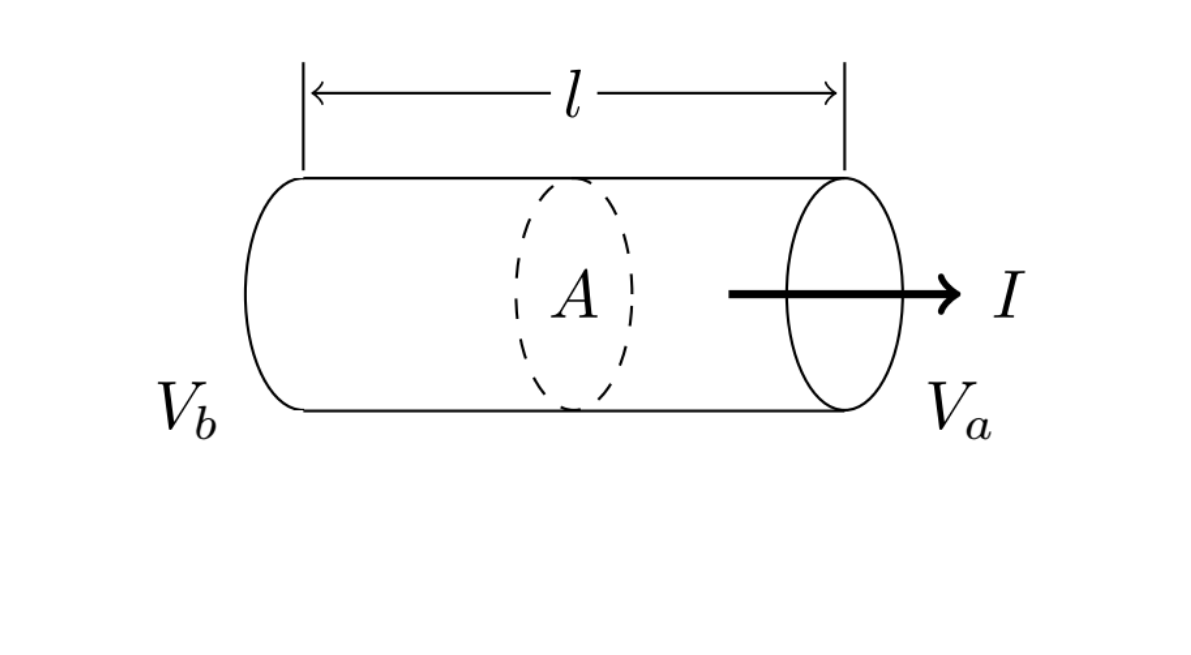
\includegraphics[width=0.4\textwidth]{./Exp2/pic/wireresistance.png}
\caption{Resistance of a uniform wire.}
\label{fig:cross-sec}
\end{figure}

The current $I$ that this potential difference produces can be obtained once we know the resistance $R$ of this wire:
\begin{equation}
	I = \frac{\Delta V}{R}
\end{equation}

The resistance of the wire is proportional to its length (the longer the wire, the ``harder" it is for electrons to travel from $b$ to $a$) and inversely proportional to its cross-sectional area (the wider the wire, the ``easier" it is for electrons to travel from $b$ to $a$):
\begin{equation}
	R = \rho \frac{l}{A}
\end{equation}

where the constant of proportionality $\rho$ is called the resistivity and is a characteristic of the material the wire is made of.

\subsection{Kirchhoff's Rules}

Simple circuits can be analyzed using the expression $V = IR$ and the rules for series and parallel combinations of resistors. Very often, however, it is not possible to reduce a circuit to a single loop. The procedure for analyzing more complex circuits is greatly simplified if we use two principles called Kirchhoff's rules.\myskip

\begin{enumerate}
	\item Junction Rule: The sum of the currents entering any junction in a circuit must equal the sum of the currents leaving that junction:
	\begin{equation}
		\sum I_{in} = \sum I_{out}
	\end{equation}
	This is basically just the statement of conservation of electric charge. For example, if we have a junction as shown in Figure \ref{fig:junction}, then we have $I_1 = I_2 + I_3$.

	\begin{figure}[h]
	\centering
	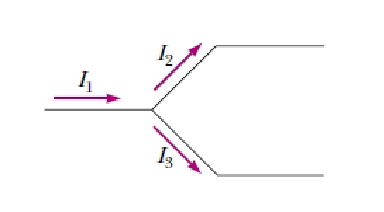
\includegraphics[width=0.3\textwidth]{./Exp2/pic/junction.png}
	\caption{A sample junction}
	\label{fig:junction}
	\end{figure}

	\item Loop Rule: The sum of the potential differences across all elements around any closed circuit loop must be zero:
	\begin{equation}
		\sum_{\text{Closed Loop}} V = 0
	\end{equation}
	This rule simply follows from conservation of energy.

\end{enumerate}

When applying Kirchhoff's second rule in practice, we imagine traveling around some loop and consider changes in electric potential, bearing in mind the following sign conventions:\myskip
\begin{itemize}
	\item If a resister is traversed in the direction of the current, the potential difference across the resistor is negative (Figure \ref{fig:signconventions}, (a))
	\item If a resistor is traversed in the direction opposite the current, the potential difference will then be positive (Figure \ref{fig:signconventions}, (b))
	\item If a source of EMF (assumed to have zero internal resistance) is traversed in the direction of the EMF (from $-$ to $+$), the potential difference will be positive (Figure \ref{fig:signconventions}, (c))
	\item If the source is traversed in the direction opposite the EMF (from $+$ to $-$), the potential difference will be negative (Figure \ref{fig:signconventions}), (d))
\end{itemize}

\begin{figure}[h]
\centering
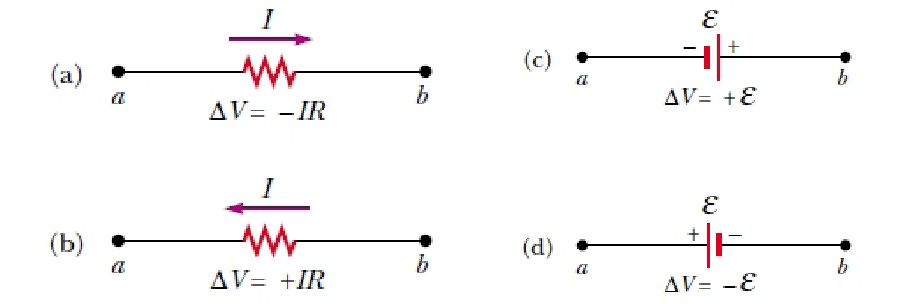
\includegraphics[width=0.6\textwidth]{./Exp2/pic/signconventions.jpg}
\caption{Sign conventions for Kirchhoff's Second Rule}
\label{fig:signconventions}
\end{figure}

In practice, for a given circuit diagram, we first label all the known and unknown quantities and assign a direction to the current in each branch of the circuit. Although the assignment of current directions is arbitrary, you must adhere rigorously to the assigned directions when applying Kirchhoff's rules. After applying Kirchhoff's rules to junctions and loops as necessary, we simply need to solve the resulting equations simultaneously for the unknown quantities. If some current turns out to be negative, that simply means that it direction is opposite to that which we assigned, but its magnitude will be correct!

\section{Procedure: Ohm's Law}
\label{sec:ohmslaw}
We will using a Multimeter to make all our measurements in this experiment. A multimeter has settings to make many different types of measurements across various ranges, so make sure that when using it, you've selected the right setting for your needs.\myskip

Choose three of the resistors that you have been given. Using the chart in Figure \ref{fig:resistancechart}, decode the resistance values and record the value in the first column of Table \ref{tab:ohmslaw}.\myskip

\begin{figure}[h]
\centering
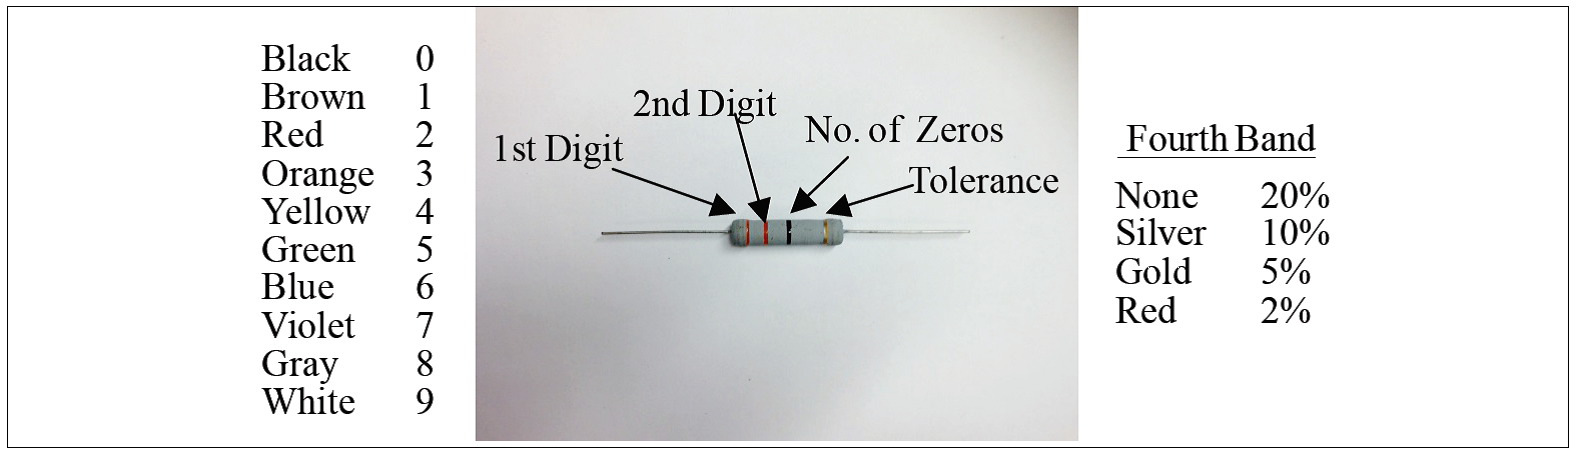
\includegraphics[width=0.8\textwidth]{./Exp2/pic/resistancechart.png}
\caption{A diagram of colorcoded resistors. (I know you can't see the color in this book)}
\label{fig:resistancechart}
\end{figure}

\subsection{Measuring Current}
To measure the current going through our resistor, we must first build an incomplete circuit! That may seem strange, but two probes of the multimeter will act as two ends of the final wire that will finish the circuit, displaying the current passing through.\myskip

\begin{enumerate}
	\item Construct the curcuit shown in Figure \ref{fig:currentpic} by pressing the leads of the resistor onto two of the springs in the Experimental Section on the Circuits Experiment Board.

	\item Set the multimeter to the 200 mA range. Connect the circuit through the multimeter and read the current that is flowing through the resistor. Record this value in the second column of Table \ref{tab:ohmslaw}.

	\begin{figure}[h]
	\centering
	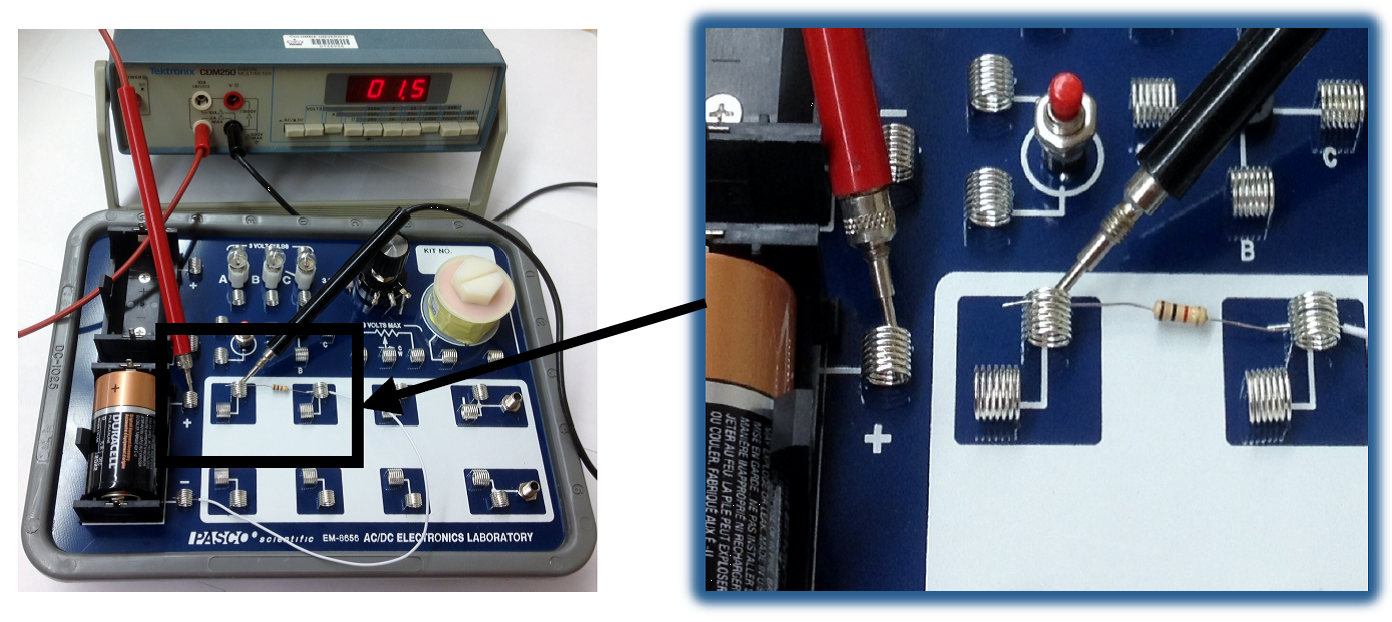
\includegraphics[width=0.8\textwidth]{./Exp2/pic/currentpic.png}
	\caption{A picture of measuring currents in circuits}
	\label{fig:currentpic}
	\end{figure}

	\item Remove the resistor and repeat the previous steps for the next two that you picked, recording everything in Table \ref{tab:ohmslaw}. Keep these three resistors handy for the next steps!

	\item What would happen if we completed our circuit with a wire and measured the current with the multimeter at the same two points? Think of Kirchhoff's laws.

\end{enumerate}

\subsection{Measuring Voltages}
Measuring voltage is different! Here we will construct a complete circuit and our two probes will tell us the potential (voltage) difference between those two positions in the system.\myskip

\begin{enumerate}
	\item Disconnect the multimeter and connect a wire from the positive lead of the battery directly into the first resistor you used as shown in Figure \ref{fig:voltpic}. Note that this completes the circuit. Change the multimeter to the $2V$ DC scale and connect the leads as shown also in that figure. Measure your voltage across the resistor and record it in Table \ref{tab:ohmslaw}.

	\begin{figure}[h]
	\centering
	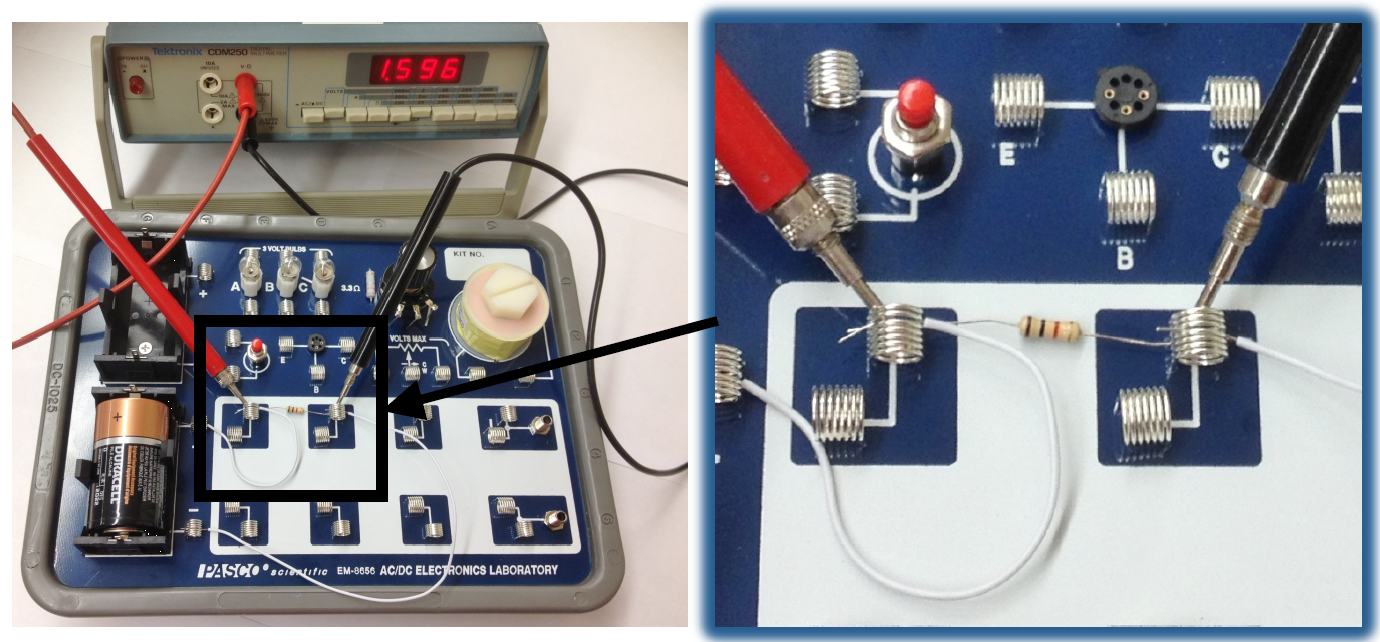
\includegraphics[width=0.8\textwidth]{./Exp2/pic/voltpic.png}
	\caption{A picture of measuring voltage in circuits.}
	\label{fig:voltpic}
	\end{figure}

	\item Repeat the last step for the remaining two resistors.

	\item For each of your datasets, calculate the ratio of voltage divided by the resistance. Record your result in the corresponding column of Table \ref{tab:ohmslaw}. Compare the values you calculate with your measured values of the current.

	\item Construct a graph of current vs. 1/resistance ($I$ vs. $\frac{1}{R}$). Include error bars from the precision of the multimeter.

	\item Does your graph form a straight line?

	\item Draw a line of best fit and determine the slope with error using LINEST.

	\item How does your slope compare to the voltage across each resistor? Do they agree within error?

\begin{table}
\begin{center}
\begin{tabular}{| c | c | c | c |}
\hline
	Resistance ($\Omega$) & Current (A) & Voltage (V) & Voltage/Resistance (V/$\Omega$ = A) \\
	\hline
	& & & \\
	\hline
	& & & \\
	\hline
	& & & \\
	\hline
\end{tabular}
\end{center}
\caption{Resistance, current and voltage measurements for Section \ref{sec:ohmslaw}.}
\label{tab:ohmslaw}
\end{table}

\end{enumerate}

\subsection{Measuring Resistances}
\label{sec:resist}
You already know the coded resistance of each of your resistors from the colored stripes, but now we will verify how accurate those are. Measuring resistance does not require a circuit at all. With your multimeter set to resistance mode, it will act as our power supply (like a battery) so touching the probes to each side of the resistor will send current through and the multimeter's display will tell us its measured resistance.\myskip

\begin{enumerate}
	\item Choose three resistors. They could be the ones from before or entirely new ones. Enter their corresponding sets of colors in Table \ref{tab:resistance}. We will refer to one as Resistor \#1, another as \#2 and the third as \#3.

	\begin{table}
		\begin{center}
			\begin{tabular}{| c | c | c | c | c |}
				\hline
				Color Bands & Coded Resistance ($\Omega$) & Measured Resistance ($\Omega$) & $\%$ Error & Tolerance \\
				\hline
				$\#1$ & & & & \\
				\hline
				$\#2$ & & & & \\
				\hline
				$\#3$ & & & & \\
				\hline
			\end{tabular}
		\end{center}
		\caption{Resistance and error Section \ref{sec:resist}.}
		\label{tab:resistance}
	\end{table}

	\item Determine the coded value of your resistors from the color code in Figure \ref{fig:resistancechart}. Enter the Tolerance value as indicated by the color of the fourth bar in the plot.

	\item Use the multimeter to measure the resistance of each of your three resistors. Enter these values in the table.

	\item Determine the percentage experimental error of each resistance value and enter in the appropriate column.
	\begin{equation}
		\text{\% Error} = \frac{|\text{Measured} - \text{Coded}|}{\text{Coded}} \times 100\%
	\end{equation}

	\item How does the \% error compare to the coded tolerance for your resistors?

\end{enumerate}

\section{Procedure: Resistors in Series and Parallel}
It is rare that we encounter circuits with just a single resistor and power source. This section will walk through how we deal with multiple resistors in different layouts.\myskip

\subsection{Series Circuits}
\begin{enumerate}

	\item Take those same three resistors from Section \ref{sec:resist}. Connect the resistors in a series circuit shown in Figure \ref{fig:voltseries} using the springs to hold the leads of the resistors together without bending them. Connect two wires to the D cell battery and carefully note which side is positive and which is negative.

	\begin{figure}[h]
	\centering
	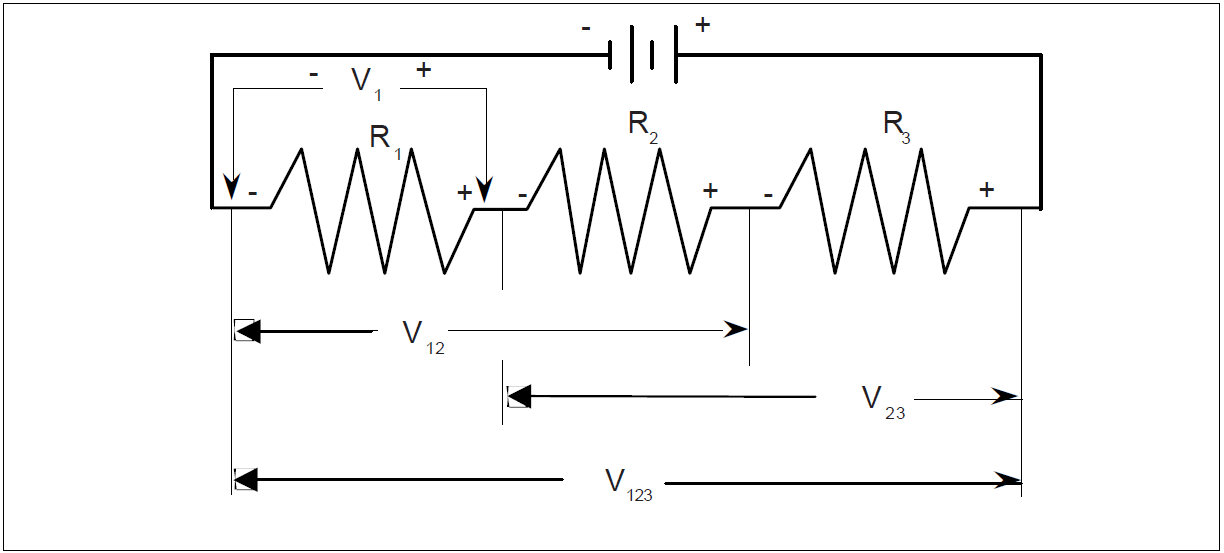
\includegraphics[width=0.9\textwidth]{./Exp2/pic/voltseries.png}
	\caption{A diagram of the series circuit}
	\label{fig:voltseries}
	\end{figure}

	\item First, disconnect the wires from the battery so we can measure the resistances along the circuit. Use the Multimeter to measure resistance of each individual resistor as well as each series combination by placing the two probes of your multimeter at the beginning and end of where you would like to measure. Make sure your multimeter is in resistance mode! Record your readings in \ref{tab:seriestable}.

	\item Reconnect your battery and measure the voltage across each resistor and each series combination of resistors. Make sure your multimeter is in voltage mode! Record your readings in \ref{tab:seriestable}.

	\begin{table}
	\begin{center}
	\begin{tabular}{| c | c | c |}
	\hline
		Resistor & Resistance ($\Omega$) & Voltage (V)\\
		\hline
		$R_1$ & &\\
		\hline
		$R_2$ & &\\
		\hline
		$R_3$ & &\\
		\hline
		$R_{12}$ & &\\
		\hline
		$R_{23}$ & &\\
		\hline
		$R_{123}$ & &\\
		\hline
	\end{tabular}
	\end{center}
	\caption{Voltage and resistance of series resistors}
	\label{tab:seriestable}
	\end{table}

	\item What is the apparent rule for total resistance when resistors are added up in series? Cite evidence from your data to support your conclusions.

	\item What is the pattern for how voltage gets distributed in a series circuit with equal resistances? Is there any relationship between the size of the resistance and the size of the resulting voltage?

\noindent Now we will modify our circuit slightly to allow us to measure current. Remember, for measuring current, the multimeter will complete the circuit. We will measure the current at four different locations following Figure \ref{fig:seriescurrent}. For a measurement at each location, we will remove the corresponding wire connector and replace it with the two probes of our multimeter. Remember to replace the wires when measuring other locations.

\begin{figure}[h]
\centering
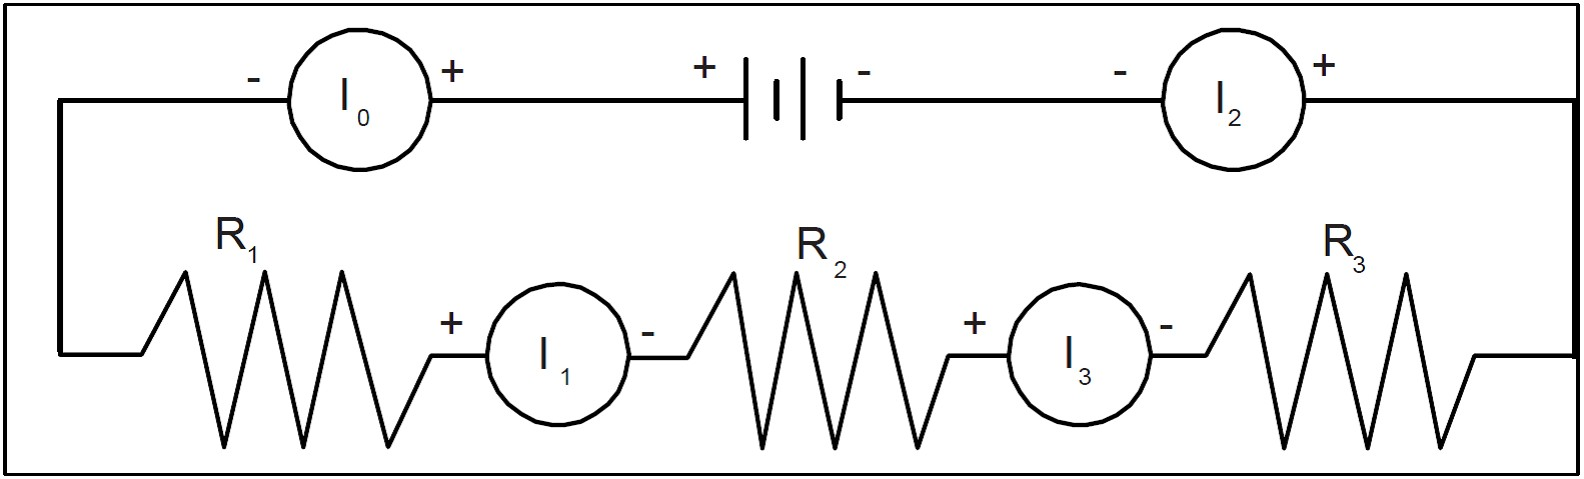
\includegraphics[width=0.9\textwidth]{./Exp2/pic/seriescurrent.jpg}
\caption{A diagram of the series circuit}
\label{fig:seriescurrent}
\end{figure}

	\item Make sure your multimeter is in current mode and measure the four currents as indicated in Figure \ref{fig:seriescurrent}. You should be using the multimeter scale which goes to a maximum of 200 mA. Be careful to observe the direction of the current in your measurements. The red probe of the meter should connect to the positive lead on the circuit and the black probe to the other. Record your results in Table \ref{tab:seriescurrent}.

	\begin{table}
	\begin{center}
	\begin{tabular}{| c | c |}
	\hline
		 & Current (A)\\
		\hline
		$I_0$ &\\
		\hline
		$I_1$ &\\
		\hline
		$I_2$ &\\
		\hline
		$I_3$ &\\
		\hline
	\end{tabular}
	\end{center}
	\caption{Current across series resistors}
	\label{tab:seriescurrent}
	\end{table}

	\item What is the pattern for how current behaves in a series circuit?

\end{enumerate}

\subsection{Parallel Circuits}
\begin{enumerate}
	\item Take the same three resistors and connect them in a parallel circuit following Figure \ref{fig:voltparallel}.

	\begin{figure}[h]
	\centering
	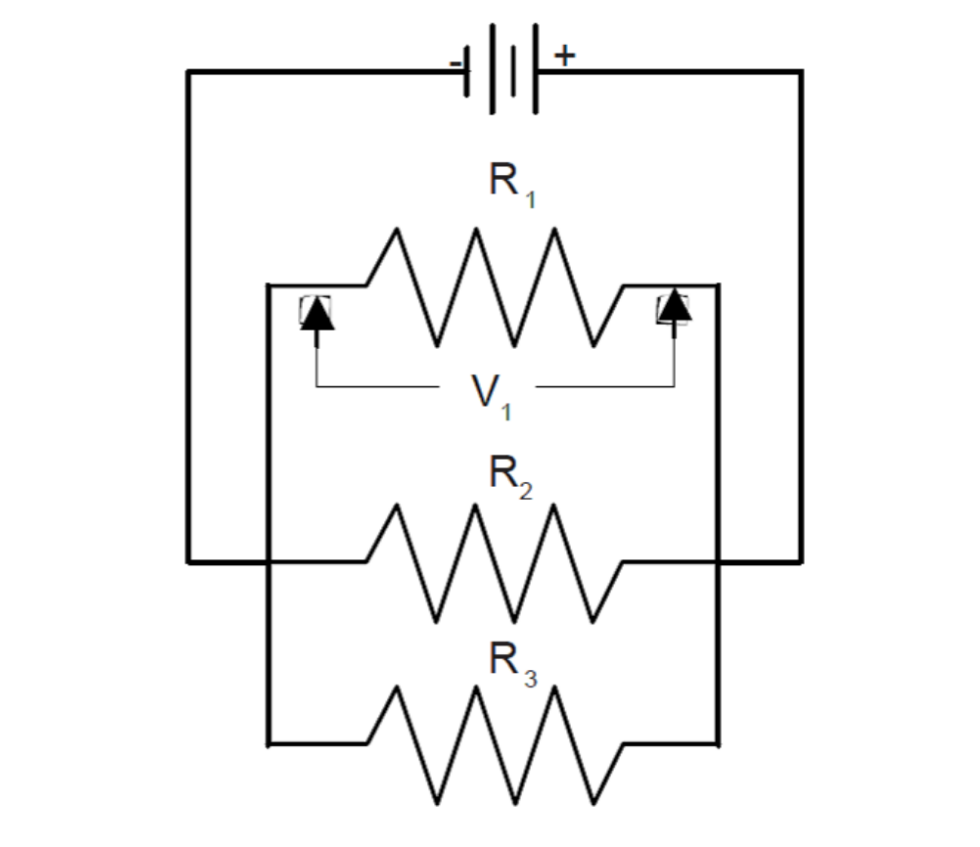
\includegraphics[width=0.4\textwidth]{./Exp2/pic/voltparallel.png}
	\caption{A diagram of the parallel circuit}
	\label{fig:voltparallel}
	\end{figure}

	\item As before, set your multimeter to resistance mode and disconnect your battery. Measure the resistance of each individual resistor as well as one across the whole parallel set of resistors (by placing your probes at the two junction points in Figure \ref{fig:voltparallel}). Record your measurements in Table \ref{tab:paralleltable}.

	\item Reconnect your battery and measure the voltage across each resistor and the parallel combination of resistors. Make sure your multimeter is in voltage mode! Record your readings in \ref{tab:paralleltable}.

	\begin{table}
	\begin{center}
	\begin{tabular}{| c | c | c |}
	\hline
		Resistor & Resistance ($\Omega$) & Voltage (V)\\
		\hline
		$R_1$ & &\\
		\hline
		$R_2$ & &\\
		\hline
		$R_3$ & &\\
		\hline
		$R_{123}$ & &\\
		\hline
	\end{tabular}
	\end{center}
	\caption{Voltage and resistance of parallel resistors}
	\label{tab:paralleltable}
	\end{table}

	\item What is the rule for total resistance when resistors are added up in parallel? Cite evidence from your data to support your conclusions.

	\item What is the pattern for how voltage distributs itself in a parallel circuit? Is there any relationship between the size of the resistance and the size of the resulting voltage?

\noindent Now we will modify our circuit again to allow us to measure current. Review the instructions from before. We will measure the current at five different locations according to Figure \ref{fig:parallelcurrent}.

\begin{figure}[h]
\centering
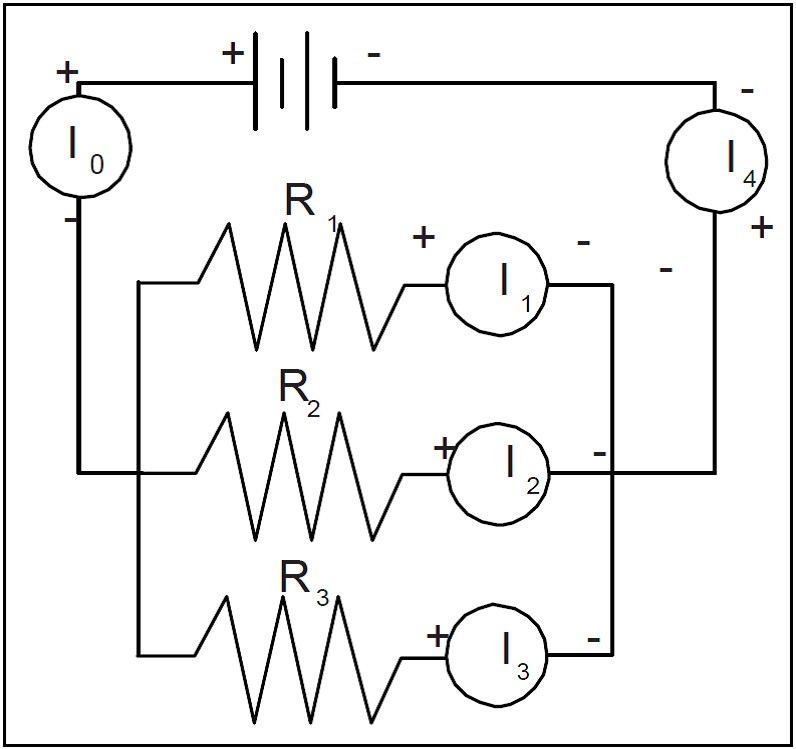
\includegraphics[width=0.4\textwidth]{./Exp2/pic/currentparallel.jpg}
\caption{A diagram of the parallel circuit}
\label{fig:parallelcurrent}
\end{figure}

	\item Make sure your multimeter is in current mode as before and measure the five currents indicated in Figure \ref{fig:parallelcurrent}. Be careful to observe the direction of the current in your measurements. Record your results in Table \ref{tab:parallelcurrent}.

	\begin{table}
	\begin{center}
	\begin{tabular}{| c | c |}
	\hline
		 & Current (A)\\
		\hline
		$I_0$ &\\
		\hline
		$I_1$ &\\
		\hline
		$I_2$ &\\
		\hline
		$I_3$ &\\
		\hline
		$I_4$ &\\
		\hline
	\end{tabular}
	\end{center}
	\caption{Current across parallel resistors}
	\label{tab:parallelcurrent}
	\end{table}

	\item Are there any patterns to the way currents behave in a parallel circuit?

\end{enumerate}
